\documentclass{article}
\usepackage{caption}
\usepackage{setspace}
\usepackage{amsmath}
\usepackage{amssymb}
\usepackage{amsthm}
\usepackage{graphicx}
\usepackage{multirow}
\usepackage{geometry}
\usepackage{listings}
\usepackage{subfigure}
\usepackage{float}
\usepackage{listings}
\usepackage{color}
\usepackage{url}
\usepackage{ctex}
\usepackage[ruled,linesnumbered]{algorithm2e}
\geometry{a4paper}
\begin{document}
\title{\textbf{Practical 3: Ant Algorithm for Solving TSP}}
\author{Yushuo Chen\\2020101918\\MAM}
\maketitle

\section*{Introduction}
In this assessment report, I am going to solve challenge B which aims to solve TSP problem using ant algorithm.
\footnote{All codes attached to homework could be found in \url{https://github.com/CyanCap/CI-code.git}.}

\section{Problem Description}
TSP problem is in order to find a minimal length closed tour that visits each city once.
My report will reveal the path which obtain the optimal distance based on dataset \textit{st70} from homework 2.
And I will compare algorithm AA (ant algorithm) and GA (genetic algorithm) solving the same TSP problem.

\section{Solution Encoding}
Since we need to obtain a cyclic path of 70 cities, we can represent one path as a permutation \textbf{e.g.} (2 3 7 6 1 5 4),
where the number 1 represents city A and number 2 represents city B etc.
Let $t$ represent a solution as this permutation, and $\mathcal{T}$ be the set of all permutations of cities set i.e.the search space.\\

Then we can calculate the Euclidean distance between each city according the locations.
\[
    D(i(x_1,y_1),\; j(x_2,y_2))=\sqrt{(x_1 - x_2)^2 + (y_1 - y_2)^2}.
\]
So the total distance during a tourment is:
\begin{align*}
    dis=[\sum_{i>=1}^{7} D(t(i),t(i+1))]+D(t(1),t(8)).
\end{align*}

\section{Objective Function And Constraint}
Obviously, we want to find the minimal of the distance $dis$, objective function is:
\begin{align*}
    t^* = arg\min_{t\in \mathcal{T}} \;dis(t).
\end{align*}
\par Moreover, there will be just a few of constraints which I can illustrate straightly.
Firstly, each solution i.e.permutation must contain all cities.
Secondly, each solution must contain a specific city only once.
So a solution is a vector of the size $1 \times n$, n is the number of cities.

\section{Models for Ant-cycle AS}
In solving this problem, I decide to use model ant-cycle ant system.
AS is developed by ACO (ant colony optimization).
It simulates the swarm of ants finding foods according the pheromones they leave.
Each ant's decision is based on a probability
\[p_{ij}^k (t) = \left\{ 
        \begin{aligned}
        &\frac{\tau_{ij}^{\alpha}(t) \eta_{ij}^{\beta}(t)}{\sum_{u\in \mathcal{N}_i^k(t)} \tau_{iu}^\alpha (t) \eta_{iu}^{\beta}(t)}, &{\rm if} \;\;j\in \mathcal{N}_i^k(t)\\
        &\qquad \qquad \quad 0, &{\rm if} \;\;j\notin  \mathcal{N}_i^k(t)
        \end{aligned} 
    \right.
\]
where $\tau_{ij}(t)$ represents the residual amount of pheromones from node $i$ to node $j$ i.e.pheromone intensity.
And  $\eta_{ij}(t)$ is the factor that represents heuristic information.
Then we should choose the way updating the pheromone as time $t$ goes by.\\
\par Firstly, we can generate the update function:
\begin{align*}
    \tau_{ij}(t+1) = (1-\rho)\cdot \tau_{ij}(t) +\sum_{k=1}^{n_k}\Delta \tau_{ij}^k(t)
\end{align*}
Secondly, since we not only need to consider the correct direction of each choice,
but also need to think of the minimal distance from node to node and the information an ant walks so far.
We use \textbf{ant-cycle AS} to represent the way pheromone deposits i.e.$\Delta \tau_{ij}^k = Q/L_k$.

\section{Algorithm Design With Pseudo Code And Parameters}
Here is my pseudo code:
\par
\begin{algorithm}[H]
    \caption{Ant-cycle Ant System}
    \KwIn{$\alpha$, $\beta$, $\rho$, $Q$, $n_k$, $\tau_0$, $\eta$}
    \KwData{locations information from \textit{st80.csv}}
    \KwResult{optimal tourment $t^*$}
    \While{stopping condition is false}{
        place $n_k$ ants randomly\;
        construct a path for $n_k$ ants\;
        compute $dis_k$\;
        reserve the best tourment\;
        evaporate and update pheromone\;
        reset all ants\;
        }
\end{algorithm}
\par
Now we should set all parameters which must fit our algorithm and problem better.
\begin{itemize}
    \item Population of ants: $n_k = 100$. 
    Population with 100 ants may perform well since amounts of ants must greater than that of destinations in nature.
    \item Decision process biases: $\alpha = 2$, $\beta = 5$.
    I want the ants to be more likely to wander randomly ($\tau^{\alpha}$) and be more creative ($\eta^{\beta}$).
    \item Factor of pheromone evaporate: $\rho = 0.2$.
    Pheromones should last long because that we want reserve some important informations after setting $\alpha$ and $\beta$.
    \item Factor indicating power of pheromone: $Q = 100$.
\end{itemize}

\section{Result And Analysis}
I obtain the final result is 
\begin{align*}
    dis_{\min} = 702.3406
\end{align*}
with tourment in variable $path\_best$.
\par
And I found that this result appeared after iteration 8, which means this algorithm perform very quickly.
Moreover, the line sees a rapid decline when it begins, and then reaches a minimum and stays in that level.
After operating such a lot of experiments, interest phenomenons happen:
algorithm usually reaches minimum but local minimum in the most of times.
\par
We can see a dramatical decrease at first, then a straight line parallel to x-axis.
As you can see, 2 figures share the same shape and similar result.
We cannot conclude more unless AS executes quickly and easy hitting (local) minimum.
\par

\begin{figure}[htbp]
    \centering
    \subfigure[experiment-1]{
        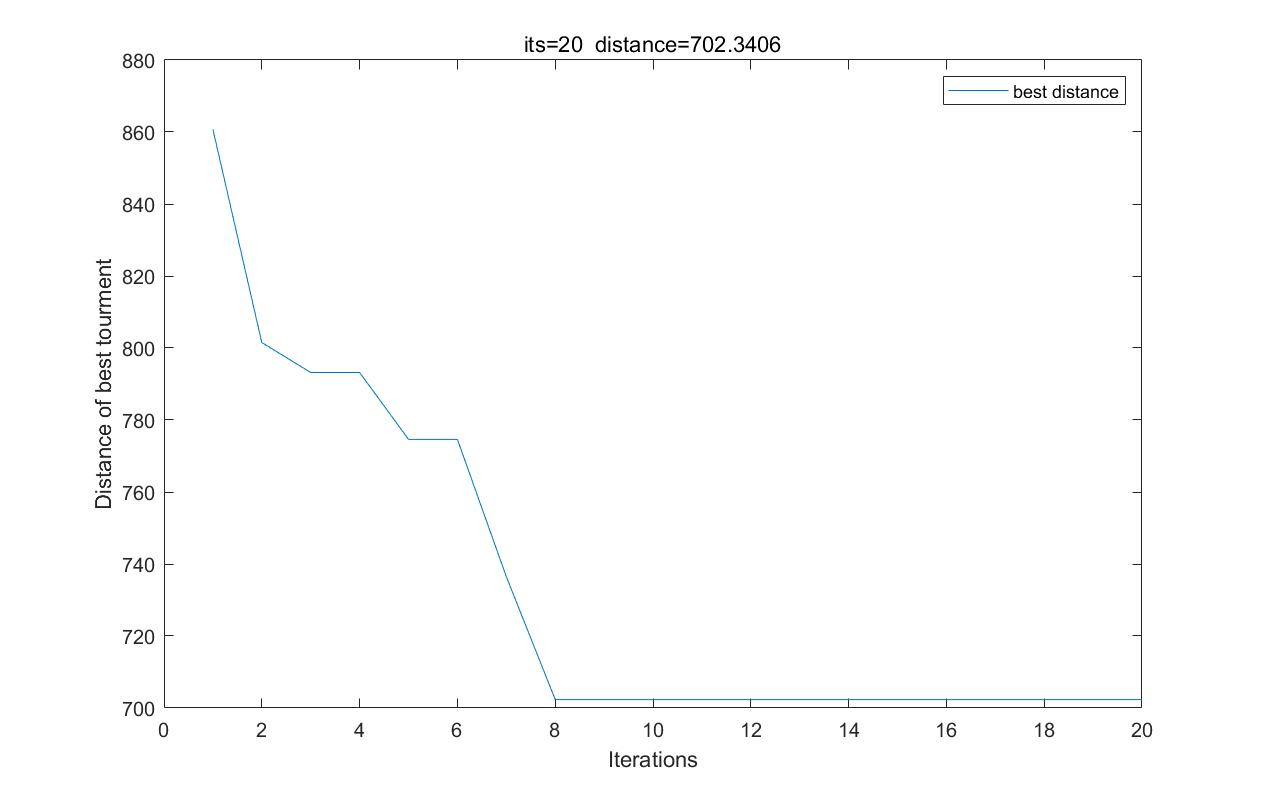
\includegraphics[scale=0.15]{1.jpg}
    }
    \subfigure[experiment-2]{
        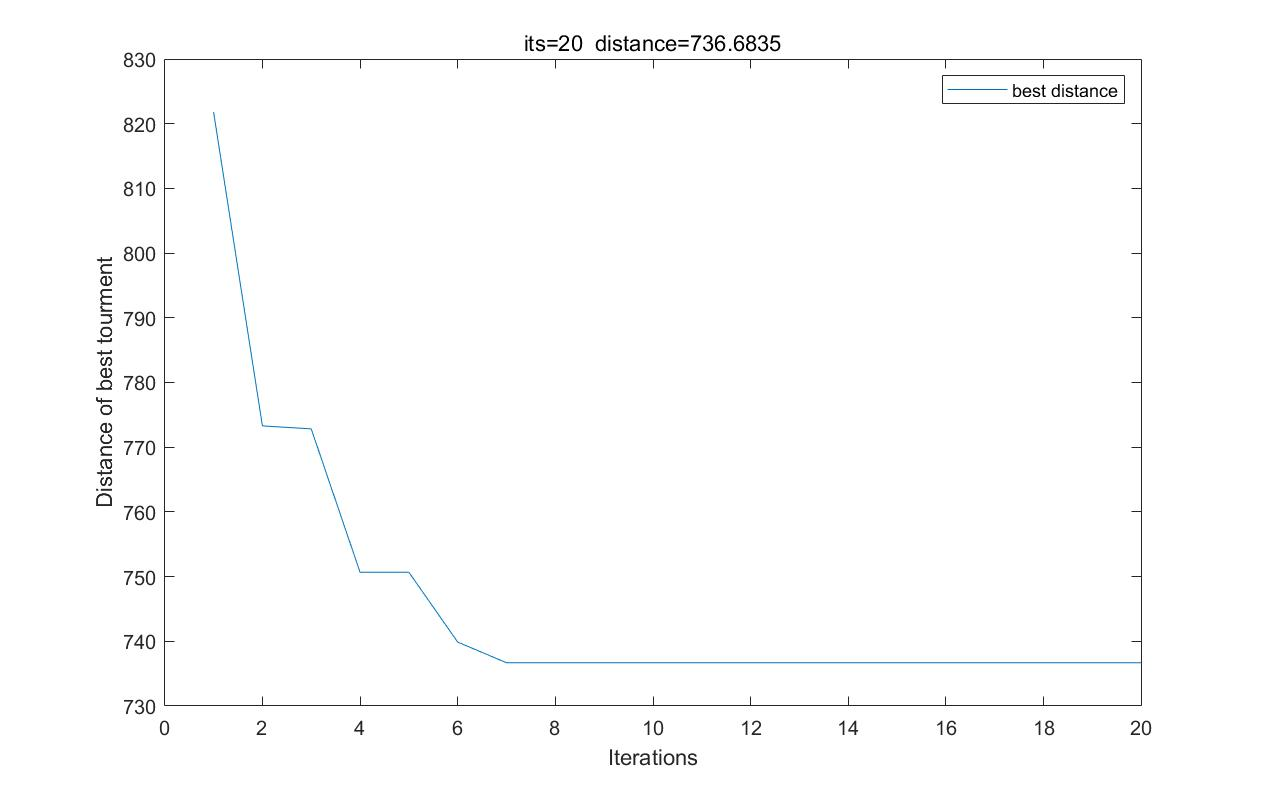
\includegraphics[scale=0.15]{2.jpg}
    }
\end{figure}

\section{More Discussions}
\begin{figure}[htbp]
    \centering
    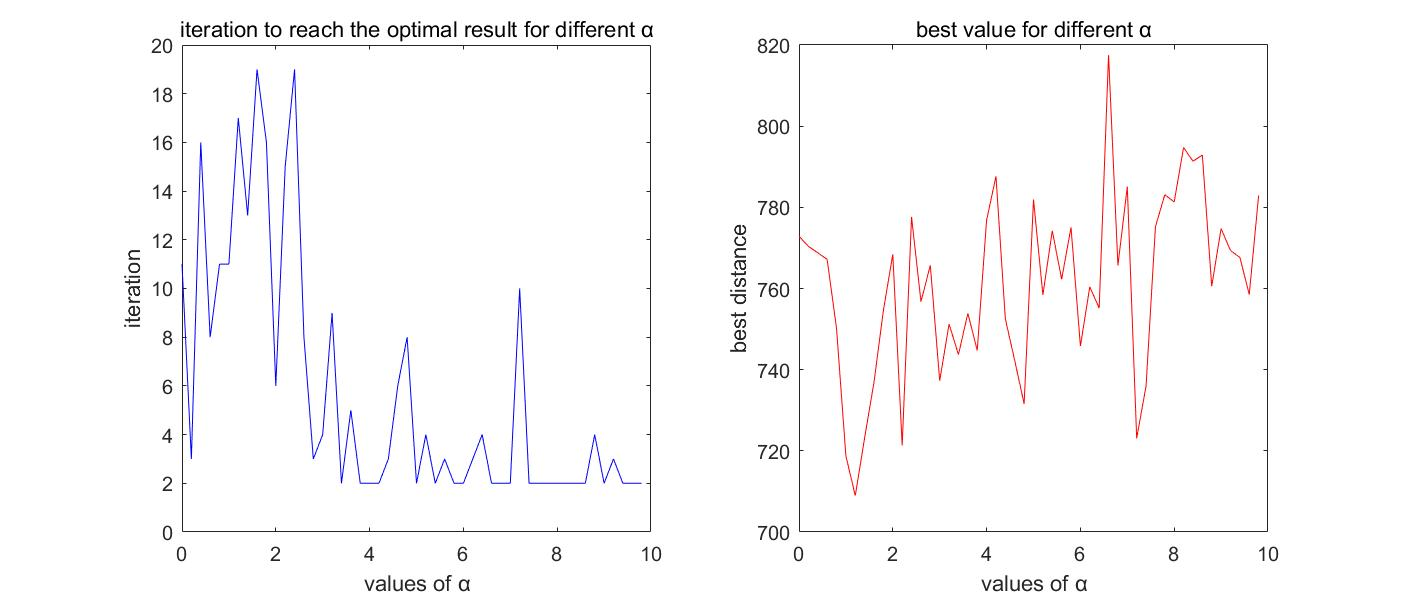
\includegraphics[scale=0.25]{3.jpg}
\end{figure}
\par   
Moreover, if we analyze effects about different $\alpha$, 
we can find that $\alpha$ needn't to be too large or small.
The left graph almost shows a convex ``几'' shape.
While the right graph has showed a increasing trade.
\par
Now we can compare a little bit of AS and GA.
In homework 2, I've designed genetic algorithm to solve same TSP problem with same dataset.
But GA has cost much more time than AS.
This difference almost could be 1000 times of cost.
And the final result is even worse than using AS.
\end{document}





